\secrel{Низкоуровневое чтение/запись \pack{SD}/MMC через
\pack{SPI}\ref{ESPI}}\secdown\label{ESD}

\cp{http://elm-chan.org/docs/mmc/mmc_e.html}

The Secure Digital Memory Card (SDC below) is the de facto standard memory card
for mobile equipments. The SDC was developped as upper-compatible to Multi Media
Card (MMC below). SDC compleant equipments can also use MMCs in most case. There
are also reduced size versions, such as RS-MMC, miniSD and microSD, with the
same function. The MMC/SDC has a microcontroller in it. The flash memory
controls (block size conversion, error correction and wearleveling - known as
FTL) are completed inside of the memory card. The data is transferred between
the memory card and the host controller as data blocks in unit of 512 bytes, so
that it can be seen as a block device like a generic harddisk drive from view
point of upper level layers.

\bigskip
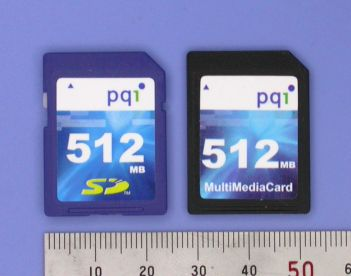
\includegraphics[height=0.5\textheight]{E/interface/SD_view.jpeg}
\bigskip

This page describes the basic knowledge and miscellaneous things that I become
aware, on using MMC/SDC with small embedded system. I believe that this
information must be a useful getting started notes for the people who is going
to use MMC/SDC on the electronics handiwork projects.

\secrel{Раскопытка}

Photo shows the contact surface of the SDC/MMC. The MMC has seven contact
pads. The SDC has nine contact pads that two additional contacts to the MMC. The
three of the contacts are assigned for power supply so that the number of
effective signals are four (MMC) and six (SDC). Therfore the data transfer
between the host and the card is done via a synchronous serial interface.

\bigskip
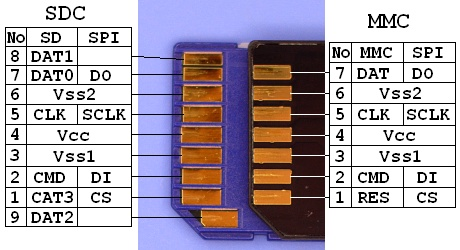
\includegraphics[height=0.5\textheight]{E/interface/SD_pads.jpeg}
\bigskip

The working supply voltage range is indicated in the operation conditions
register (OCR) and it should be read and comfirmed the operating voltage range.
However, the supply voltage can be fixed to 3.0/3.3 volts because the all
MMC/SDCs work at supply voltage of 2.7 to 3.6 volts at least. Do not supply 5.0
volts to the card, or the card is damaged instantly. The current consumption on
write operation can reach up to some ten miliamperes, so that the host system
should consider to supply 100 miliamperes to tha card.

\secrel{Режим SPI}\secdown

This document describes the SPI mode to control the MMC/SDCs. The SPI mode is an
alternative operating mode that defined to use the MMC/SDCs without native host
interface. The communication protocol of the SPI mode is a little simple
compared to its native operating mode. The MMC/SDC can be attached to the most
microcontrollers via a generic SPI interface or GPIO ports. Therefore the SPI
mode is suitable for low cost embedded applications with no native host
interface is available. There are four different SPI modes, 0 to 3, depends on
clock phase and polarity. Mode 0 is defined for SDC. For the MMC, it is not the
SPI timing, both latch and shift actions are defined with rising edge of the
SCLK, but it seems to work at mode 0 in the SPI mode. Thus the Mode 0 (CPHA=0,
CPOL=0) is the proper setting to control MMC/SDC, but mode 3 (CPHA=1, CPOL=1)
also works as well in most case.

\bigskip
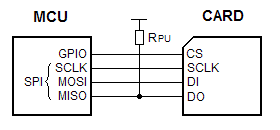
\includegraphics[height=0.3\textheight]{E/interface/SD_conn.png}
\bigskip

\secrel{Команда и ответ}

In SPI mode, the data direction on the signal lines are fixed and the data is
transferred in byte oriented serial communication. The command frame from host
to card is a fixed length packet that shown below. The card is ready to receive
a command frame when it drives DO high. After a command frame is sent to the
card, a response to the command (R1, R2, R3 or R7) is sent back from the card.
Because the data transfer is driven by serial clock generated by host
controller, the host controller must continue to read data, send a 0xFF and get
received byte, until a valid response is detected. The DI signal must be kept
high during read transfer (send a 0xFF and get the received data). The response
is sent back within command response time (NCR), 0 to 8 bytes for SDC, 1 to 8
bytes for MMC. The CS signal must be driven high to low prior to send a command
frame and held it low during the transaction (command, response and data
transfer if exist). The CRC feature is optional in SPI mode. CRC field in the
command frame is not checked by the card.

\bigskip
\noindent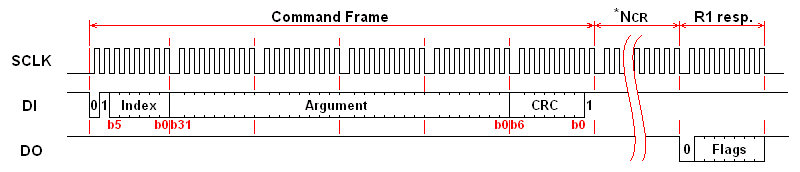
\includegraphics[width=0.95\textwidth]{E/interface/SD_cmd.png}
\bigskip

\secrel{Набор команд SD SPI}

Each command is expressed in abbreviation like \verb|GO_IDLE_STATE| or CMD<n>,
<n> is the number of the command index and the value can be 0 to 63. Following table
describes only commands that to be usually used for generic read/write and card
initialization. For details on all commands, please refer to spec sheets from
MMCA and SDCA.

\clearpage\noindent
{\footnotesize
\begin{tabular}{l l l l l l}
\hline
Command & Argument	& Response	& Data	& Abbreviation	& Description \\
Index &&&&&	\\
\hline

CMD0&	None(0)&	R1&	No&	GO\_IDLE\_STATE&	Software reset.\\
CMD1&	None(0)&	R1&	No&	SEND\_OP\_COND&	Initiate initialization process.\\
ACMD41(*1)&	*2&	R1&	No&	APP\_SEND\_OP\_COND&	For only SDC.\\
&&&&& Initiate
initialization process.\\
CMD8&	*3&	R7&	No&	SEND\_IF\_COND&	For only SDC V2. Check voltage range.\\
CMD9&	None(0)&	R1&	Yes&	SEND\_CSD&	Read CSD register.\\
CMD10&	None(0)&	R1&	Yes&	SEND\_CID&	Read CID register.\\
CMD12&	None(0)&	R1b&	No&	STOP\_TRANSMISSION&	Stop to read data.\\
CMD16&	Block &	R1&	No&	SET\_BLOCKLEN&	Change R/W block size.\\
&length[31:0]\\
CMD17&	Address[31:0]&	R1&	Yes&	READ\_SINGLE\_BLOCK&	Read a block.\\
CMD18&	Address[31:0]&	R1&	Yes&	READ\_MULTIPLE\_BLOCK&	Read multiple blocks.\\
CMD23&	Number of &	R1&	No&	SET\_BLOCK\_COUNT&	For only MMC.\\
&blocks[15:0]&&&&Define
number of blocks to transfer\\
&&&&& with next multiblock r/w command.\\
ACMD23(*1)&	Number of &	R1&	No&	SET\_WR\_BLOCK\_ERASE\_COUNT&	For
only SDC.\\
&blocks[22:0]&&&&Define number of blocks to pre-erase\\
&&&&&with next multi-block write
command.\\
CMD24&	Address[31:0]&	R1&	Yes&	WRITE\_BLOCK&	Write a block.\\
CMD25&	Address[31:0]&	R1&	Yes&	WRITE\_MULTIPLE\_BLOCK&	Write multiple blocks.\\
CMD55(*1)&	None(0)&	R1&	No&	APP\_CMD&	Leading command of ACMD<n>\\
&&&&& command.\\
CMD58&	None(0)&	R3&	No&	READ\_OCR&	Read OCR.\\

\hline
\end{tabular}\bigskip

(1) ACMD<n> means a command sequense of CMD55-CMD<n>

(2) Rsv(0)[31], HCS[30], Rsv(0)[29:0]

(3) Rsv(0)[31:12], Supply Voltage(1)[11:8], Check Pattern(0xAA)[7:0]
}
\clearpage

\secrel{Ответ по SPI}

There are some command response formats, R1, R2, R3 and R7, depends on the
command index. A byte of response, R1, is returned for most commands. The bit
field of the R1 response is shown in right image, the value 0x00 means
successful. When any error occured, corresponding status bit in the response
will be set. The R3/R7 response (R1 + trailing 32-bit data) is for only CMD58
and CMD8.

\bigskip
\noindent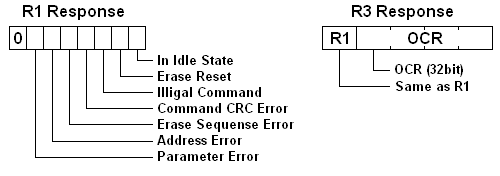
\includegraphics[height=0.3\textheight]{E/interface/SD_R1R3.png}
\bigskip

Some commands take a time longer than NCR and it responds R1b. It is an R1
response followed by busy flag (DO is driven to low as long as internal process
is in progress). The host controller should wait for end of the process until DO
goes high (a 0xFF is received).

\secup

\secrel{Процедура инициализации}\secdown

After power on reset, MMC/SDC enters its native operating mode. To put it SPI
mode, follwing procedure must be performed like this flow.

\secrel{Подача питания или вставка карты в держатель}

After supply voltage reached 2.2 volts, wait for one millisecond at least. Set
SPI clock rate between 100 kHz and 400 kHz. Set DI and CS high and apply 74 or
more clock pulses to SCLK. The card will enter its native operating mode and go
ready to accept native command.

\secrel{Программный сброс}

Send a CMD0 with CS low to reset the card. The card samples CS signal on a CMD0
is received successfully. If the CS signal is low, the card enters SPI mode and
responds R1 with In Idle State bit (0x01). Since the CMD0 must be sent as a
native command, the CRC field must have a valid value. When once the card enters
SPI mode, the CRC feature is disabled and the CRC is not checked by the card, so
that command transmission routine can be written with the hardcorded CRC value
that valid for only CMD0 and CMD8 with the argument of zero. The CRC feature can
also be switched with CMD59.

\secrel{Инициализация}

In idle state, the card accepts only CMD0, CMD1, ACMD41,CMD58 and CMD59. Any
other commands will be rejected. In this time, read OCR register and check
working voltage range of the card. In case of the system sypply voltage is out
of working voltage range, the card must be rejected. Note that all cards work at
supply voltage range of 2.7 to 3.6 volts at least, so that the host contoller
needs not check the OCR if supply voltage is in this range. The card initiates
the initialization process when a CMD1 is received. To detect end of the
initialization process, the host controller must send CMD1 and check the
response until end of the initialization. When the card is initialized
successfuly, In Idle State bit in the R1 response is cleared (R1 resp changes
0x01 to 0x00). The initialization process can take hundreds of milliseconds
(large cards tend to longer), so that this is a consideration to determin the
time out value. After the In Idle State bit cleared, generic read/write commands
will able to be accepted.

Because ACMD41 instead of CMD1 is recommended for SDC, trying ACMD41 first and
retry with CMD1 if rejected, is ideal to support both type of the cards.

The SCLK rate should be changed to fast as possible to maximize the read/write
performance. The TRAN\_SPEED field in the CSD register indicates the maximum
clock rate of the card. The maximum clock rate is 20MHz for MMC, 25MHz for SDC
in most case. Note that the clock rate will able to be fixed to 20/25MHz in SPI
mode because there is no open-drain condition that restricts the clock rate.

The initial read/write block length can be set 1024 on 2GB cards, so that the
block size should be re-initialized to 512 with CMD16 to work with FAT file
system.

\secrel{Инициализация SDHC карт}

After the card enters idle state with a CMD0, send a CMD8 with argument of
0x000001AA and correct CRC prior to initialization process. If the CMD8 is
rejected with illigal command error (0x05), the card is SDC version 1 or MMC
version 3. If accepted, R7 response (R1(0x01) + 32-bit return value) will be
returned. The lower 12 bits in the return value 0x1AA means that the card is SDC
version 2 and it can work at voltage range of 2.7 to 3.6 volts. If not the case,
the card should be rejected. And then initiate initialization with ACMD41 with
HCS flag (bit 30). After the initialization completed, read OCR register with
CMD58 and check CCS flag (bit 30). When it is set, the card is a high-capacity
card known as SDHC/SDXC. The data read/write operations described below are
commanded in block addressing insted of byte addressing. The size of data block
at block addressing mode is fixed to 512 bytes.

\secup

\secrel{Data Transfer}\secdown

\secrel{Data Packet and Data Response}

In a transaction with data transfer, one or more data blocks will be
sent/received after command response. The data block is transferred as a data
packet that consist of Token, Data Block and CRC. The format of the data packet
is showin in right image and there are three data tokens. Stop Tran token is to
terminate a multiple block write transaction, it is used as single byte packet
without data block and CRC.

\bigskip
\noindent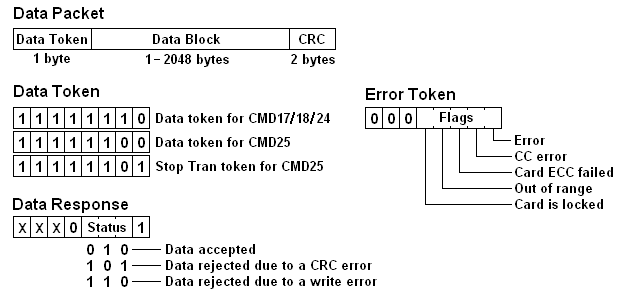
\includegraphics[height=0.5\textheight]{E/interface/SD_data.png}
\bigskip

\secrel{Single Block Read}

The argument specifies the location to start to read in unit of byte or block.
The sector address in LBA specified by upper layer must be scaled properly. When
a CMD17 is accepted, a read operation is initiated and the read data block will
be sent to the host. After a valid data token is detected, the host controller
receives following data field and CRC. The CRC bytes must be received even if it
is not needed. If any error occured during the read operation, an error token
will be returned instead of data packet.

\bigskip
\noindent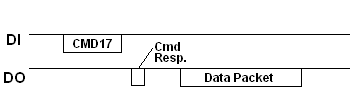
\includegraphics[height=0.2\textheight]{E/interface/SD_SBR.png}
\bigskip

\secrel{Multiple Block Read}

The CMD18 is to read multiple blocks in sequense from the specified location.
The read operation continues as open-ended. To terminate the transaciton, send a
CMD12 to the card. The received byte immediataly following CMD12 is a stuff
byte, it should be discarded before receive the response of the CMD12. For MMC,
if number of transfer blocks has been sepecified by CMD23 prior to CMD18, the
read transaction is initiated as a pre-defined multiple block transfer and the
read operation is terminated at last block transfer.

\bigskip
\noindent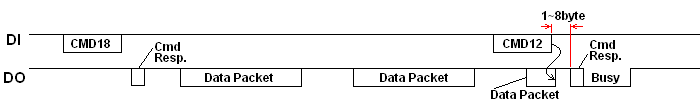
\includegraphics[height=0.2\textheight]{E/interface/SD_MBR.png}
\bigskip

\secrel{Single Block Write}

The Single Block Write writes a block to the card. After a CMD24 is accepted,
the host controller sends a data packet to the card. The packet format is same
as block read operations. Most cards cannot change write block size and it is
fixed to 512. The CRC field can have any fixed value unless the CRC function is
enabled. The card responds a Data Response immediataly following the data packet
from the host. The Data Response trails a busy flag and host controller must
wait until the card goes ready.

In principle of the SPI mode, the CS signal must be kept asserted during a
transaction. However there is an exception to this rule. When the card is busy,
the host controller can deassert CS to release SPI bus for any other SPI
devices. The card will drive DO low again when reselected during internal
process is in progress. Therefore a preceding busy check, check if card is busy
prior to each command and data packet, instead of post wait can eliminate waste
wait time. In addition the internal write process is initiated a byte after the
data response, this means eight clocks are required to initiate internal write
operation. The state of CS signal during the eight clocks can be either low or
high, so that it can be done by bus release process described below.

\bigskip
\noindent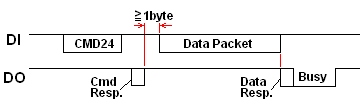
\includegraphics[height=0.2\textheight]{E/interface/SD_SBW.png}
\bigskip

\secrel{Multiple Block Write}

The Multiple Block Read command writes multiple blocks in sequense from the
specified location. After a CMD25 is accepted, the host controller sends one or
more data packets to the card. The packet format is same as block read
operations except for Data Token. The write operation continues until terminated
with a Stop Tran token. The busy flag will output after each data block and Stop
Tran token. For MMC, the number of blocks to write can be pre-defined by CMD23
prior to CMD25 and the write transaction is terminated at last data block. For
SDC, number of sectors to pre-erased at start of write transaction can be
specified by ACMD23 prior to CMD25. A Stop Tran token is always required to
treminate the write transaction. It can also be terminated at smaller or larger
than pre-erased blocks but the content of the pre-erased and not transferred
blocks are undefined.

\bigskip
\noindent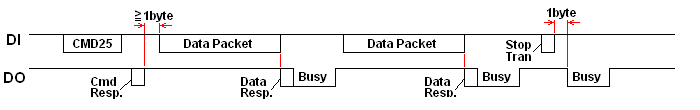
\includegraphics[height=0.2\textheight]{E/interface/SD_MBW.png}
\bigskip

\secrel{Reading CSD and CID}

These are same as Single Block Read except for the data block length. The CSD
and CID are sent to the host as 16 byte data block. For details of the CMD, CID
and OCR, please refer to the MMC/SDC specs.

\secup

\secrel{Cosideration to Bus Floating and Hot Insertion}

Any signals that can be floated should be pulled low or high properly via a
resister. This is a generic design rule on MOS devices. Because DI and DO are
normally high, they should be pulled-up. According to SDC/MMC specs, from 50k to
100k ohms is recommended to the value of pull-up registers. However the clock
signal is not mentioned in the SDC/MMC specs because it is always driven by host
controller. When there is a possibility of floating, it should be pulled to the
normal state, low.

\bigskip
\noindent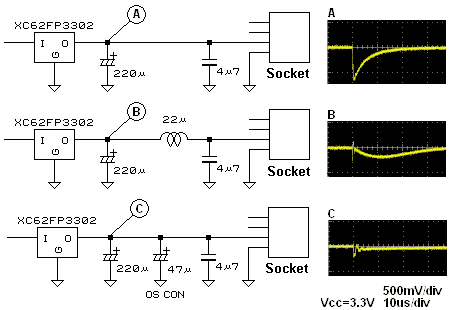
\includegraphics[height=0.7\textheight]{E/interface/SD_bus.png}
\bigskip

The MMC/SDC can hot insertion/removal but some considerations to the host
circuit are needed to avoid an incorrect operation. For example, if the system
power supply (Vcc) is tied to the card socket directly, the Vcc will dip at the
instant of contact closed due to a charge current to the capacitor that built in
the card. 'A' in the right image is the scope view and it shows that occureing a
voltage dip of about 600 millivolts. This is a sufficient level to trigger a
brown out detector. 'B' in the right image shows that an inductor is inserted to
block the surge current, the voltage dip is reduced to 200 millivoits. A low ESR
capacitor, such as OS-CON, can eliminate the voltage dip dratiscally like shown
in 'C'. However the low ESR capacitor can cause an oscillation of LDO regulator.

\secrel{Cosideration on Multi-slave Configuration}

In the SPI bus, each slave device is selected with separated CS signals, and
plural devices can be attached to an SPI bus. Generic SPI slave device
drives/releases its DO signal by CS signal asynchronously to share an SPI bus.
However MMC/SDC drives/releases DO signal in synchronising to the SCLK. This
means there is a posibility of bus conflict with MMC/SDC and any other SPI
slaves that attached to an SPI bus. Right image shows the drive/release timing
of the MMC/SDC (the DO signal is pulled to 1/2 vcc to see the bus state).
Therefore to make MMC/SDC release DO signal, the master device must send a byte
after CS signal is deasserted.

\bigskip
\noindent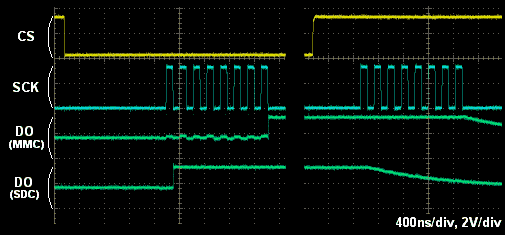
\includegraphics[height=0.5\textheight]{E/interface/SD_muslave.png}
\bigskip

\secrel{How Fast SPI Mode Can Work?}

MMC/SDC can work at the clock frequency upto 20/25 MHz. Of course all native
interfaces guarantee to work at the maximum clock frequency. However generic SPI
interface integrated in the microcontrollers may not work at high clock
frequency due to a timing issue. Right image shows the timing diagram of the SPI
interface. In SPI mode 0/3, the data is shifted out by falling edge of the SCLK
and latched by next rising edge. td is the SCLK to DO propagation delay at the
SDC, 14ns maximum. tsu is the minimum setup time of the MISO input. Therefore
the maximum allowable SCLK frequency can be calculated by:

\begin{equation}
F_{SCLK}(max) = 0.5 / (t_{d} + t_{su})
\end{equation}

Some microcontrollers I have used are limited the allowable SCLK frequency
around 10 MHz by the timing specs.

\bigskip
\noindent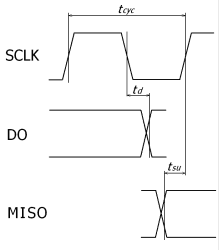
\includegraphics[height=0.5\textheight]{E/interface/SD_timing.png}
\bigskip

\secrel{File System}

The file system used on the MMC/SDC is FAT. The MMC/SDC specifications define
the FAT type as: FAT12 for 64MB or smaller cards, FAT16 for 128MB to 2GB cards,
FAT32 for 4GB to 32GB cards and exFAT for 64GB to 2TB cards. Only an FAT volume
can be exist on the card with FDISK partitioning rule and no patition table like
floppy disk is not allowed. Of course different file system other than the
MMC/SDC specifications define will able to be used as generic storage media for
PCs. However such the illigal format cards can not be recognized with home
equipments.

\secrel{Optimization of Write Performance}\secdown

Most MMC/SDC employs NAND Flash Memory as a memory array. The NAND flash memory
is cost effective and it can read/write large data fast, but on the other hand,
there is a disadvantage that rewriting a part of data is inefficient. Generally
the flash memory requires to erase existing data before write a new data, and
minimum unit of erase operation (called erase block) is larger than write block
size. The typical NAND flash memory has a block size of 512/16K bytes for
write/erase operation, and recent monster card employs large block chip
(2K/128K). This means that rewriting entire data in the erase block is done in
the card even if write only a sector (512 bytes).

\secrel{Benchmark}

I examined the read/write performance of some MMC/SDC with a cheap 8 bit MCU
(ATmega64 @9.2MHz) on the assumption that an embedded system with limited memory
size. For reason of memory size, write() and read() ware performed in 2048 bytes
at a time. The result is: Write: 77kB/sec, Read: 328kB/sec on the 128MB SDC,
Write: 28kB/sec, Read: 234kB/sec on the 512MB SDC and Write: 182kB/sec, Read:
312kB/sec on the 128MB MMC.

Therefor the write performance of the 512MB SDC was very poor that one third
value of 128MB SDC. Generally the read/write performance of the mass storage
device increases proportional to its recording density, however it sometimes
appears a tendency of opposite on the memory card. As for the MMC, it seems to
be several times faster than SDC, it is not bad performance. After that time, I
examined some SDCs supplied from different makers, and I found that PQI's SDC
was as fast as Hitachi's MMC but Panasonic's and Toshiba's one was very poor
performances.

\secrel{Erase Block Size}

To analys detail of write operation, busy time (number of polling cycles) after
sent a write data is typed out to console in the low level disk write function.
Multiple numbers on a line indicates data blocks and a Stop Tran token that
issued by a multiple block write transaction.

In resulut of the analysis, there is a different of internal process between
128MB SDC and 512MB SDC. The 128MB SDC rewrites erase block at end of the
mutiple block write transaction. The 512MB SDC seems have 4K bytes data buffer
and it rewrites erase block every 4K bytes boundary. Therefor it cannot compared
directly but the processing time of rewriting an erase block can be read 3800
for 128MB SDC and the 512MB SDC taeks 30000 that 8 times longer than 128MB SDC.
Judging from this resulut, it seems the 128MB SDC uses a small block chip and
the 512MB SDC uses a large block or MLC chip. Ofcourse the larger block size
decreases the performance on pertial block rewriting. In 512MB SDC, only an area
that 512K bytes from top of the memory is relatively fast. This can be read from
write time in close(). It might any special processing is applied to this area
for fast FAT accsess.

\secrel{Improving Write Performance}

To avoid this bottleneck and increase the write performance, number of blocks
per write transaction must be large as possible. Of course all layers between
the application and the media must support multiple sector write feature. For
low level SDC/MMC write function, it should inform number of write sectors to
the card prior to the write transaction for efficient internal write process.
This method called `pre-defined multiple block write'. The pre-definition
command is not the same between MMC (CMD23) and SDC (ACMD23).

\bigskip
\noindent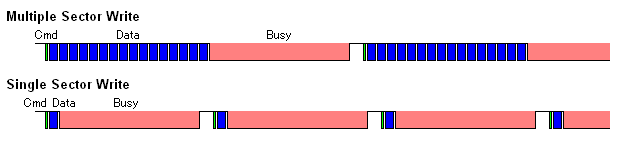
\includegraphics[height=0.3\textheight]{E/interface/SD_perf.png}
\bigskip

The memory cards are initially patitioned and formatted to align the allocation
unit to the erase block. When re-patition or re-format the memory card with a
device that not compliant to MMC/SDC (this is just a PC) with no care, the
optimization will be broken and the write performance might be lost. I tried to
re-format 512MB SDC in FAT32 with a PC, the write performance measured in file
copy was lowerd to one several. Therefore the re-formatting the card should be
done with MMC/SDC compliant equipments rather than PC.

\secup

\secup
